%% ============================================================
%% Section : Configuration de la Plateforme ST ChatGPT
%% Fichier séparé pour permettre le repositionnement dans le rapport
%% Intégré au Chapitre 4 (Réalisation et Implémentation) via \input
%% ============================================================

\section{Configuration de la Plateforme ST ChatGPT}
\label{chap:configuration}

\textit{\small\textbf{\textcolor{stblue}{Phase CRISP-DM :}} cette section couvre la phase \textit{Deployment} (mise en production sur la plateforme ST ChatGPT).}\par\smallskip

Cette section détaille la configuration de la persona \textbf{ST GitHub Analyzer} sur la plateforme ST ChatGPT et les justifications de chaque paramètre.

\subsection{Architecture de la Plateforme}

La plateforme ST ChatGPT est un service Azure OpenAI interne déployé par STMicroelectronics. Elle permet de créer des \textbf{personas} --- des agents conversationnels spécialisés --- équipés de deux types d'outils :

\begin{itemize}
  \item \textbf{KB (Knowledge Base)} : recherche dans une base de connaissances structurée
  \item \textbf{Persona-as-a-Tool} : appel à un autre agent comme fallback
\end{itemize}

\subsection{Configuration du Tool KB}

\subsubsection{Paramètres Retenus}

\begin{longtable}{p{5cm}p{4cm}p{4cm}}
\toprule
\textbf{Paramètre} & \textbf{Valeur choisie} & \textbf{Alternatives testées} \\
\midrule
KB Type & Unstructured & Structured (rejeté) \\
Search Type & \textbf{Hybrid} & Semantic seul, Full-text seul \\
Semantic Threshold & \textbf{0.55} (S0 courant) / \textbf{0.45} (S1 candidat) & 0.55, 0.45, 0.65 \\
Semantic Max Doc Count & \textbf{25} (S0) / \textbf{35} (S1) & 15, 18, 25, 35 \\
Full-text Max Doc Count & \textbf{12} & 5, 8, 20 \\
Tool fallback & \textbf{NovaX} restrictif & Fallback permissif (rejeté) \\
Modèle LLM & GPT-5.1 & GPT-4o (précédent) \\
\bottomrule
\end{longtable}

\textbf{Lecture opérationnelle} : la configuration S0 reste le point d'équilibre courant, car elle combine une bonne stabilité (QI=65) et un volume documentaire maîtrisé. La configuration S1 obtient le meilleur score mesuré (QI=66) en augmentant le rappel ; elle est donc le candidat prioritaire pour la configuration finale, sous réserve de validation du test complet en cours.

\subsubsection{Justification : Recherche Hybride}

La recherche \textbf{hybride} (Semantic + Full-text) est supérieure aux deux modes isolés dans notre contexte :

\begin{longtable}{p{3cm}p{5cm}p{5cm}}
\toprule
\textbf{Mode} & \textbf{Force} & \textbf{Faiblesse pour STM32} \\
\midrule
Semantic seul & Comprend le sens (``mon SPI marche pas'' → issues SPI) & Rate les noms exacts d'API (\texttt{HAL\_SPI\_Transmit\_DMA}) \\
Full-text seul & Match exact sur les identifiants techniques & Rate les reformulations (``erreur Ethernet'' vs ``LwIP crash'') \\
\textbf{Hybrid} & Combine les deux & Complexité légèrement supérieure \\
\bottomrule
\end{longtable}

\textbf{Résultat mesuré} : sur le benchmark complet de 96 questions, la recherche hybride surpasse les configurations mono-mode. Le semantic-only (S5) atteint 41/100 et le fulltext-heavy (S4) 47/100, alors que les stratégies hybrides équilibrées atteignent 63--66/100. Le résultat confirme que les questions STM32 combinent deux signaux complémentaires : des formulations naturelles (``problème LoRa join'', ``DMA corruption'') et des identifiants exacts (\texttt{HAL\_SPI\_Transmit\_DMA}, \texttt{NUCLEO-H743ZI}, noms de fichiers). Une stratégie purement sémantique perd les ancres exactes ; une stratégie trop full-text perd les reformulations.

\subsubsection{Justification : Seuil Sémantique à 0.55}
\label{sec:seuil_semantique}

Le \textbf{seuil sémantique} (Semantic Threshold) est le score minimum de similarité qu'un document doit atteindre pour être retourné par la recherche sémantique. Un score de 1.0 signifie une correspondance parfaite, 0.0 aucune similarité. Ce seuil contrôle directement le compromis entre \textbf{rappel} (ne rien rater) et \textbf{précision} (pas de bruit).

Le seuil de 0.55 a d'abord été calibré empiriquement sur les campagnes H7. La campagne multi-séries de juin 2026 a ensuite comparé six stratégies sur 96 questions :

\begin{longtable}{p{2cm}p{2cm}ccccp{4.3cm}}
\toprule
\textbf{Stratégie} & \textbf{Search} & \textbf{Thr.} & \textbf{Sem. docs} & \textbf{FT docs} & \textbf{QI} & \textbf{Interprétation} \\
\midrule
S0 Current & Hybrid & 0.55 & 25 & 12 & 65 & Équilibre précision/rappel courant \\
\textbf{S1 Recall+} & Hybrid & 0.45 & 35 & 15 & \textbf{66} & Meilleur score ; capte plus de cas marginaux \\
S2 Precision+ & Hybrid & 0.65 & 18 & 8 & 63 & Moins de bruit mais plus de faux négatifs \\
S3 Semantic-heavy & Hybrid & 0.55 & 35 & 6 & 51 & Trop peu d'ancrage exact API/fichiers \\
S4 Fulltext-heavy & Hybrid & 0.55 & 15 & 20 & 47 & Trop dépendant des mots exacts \\
S5 Semantic-only & Semantic & 0.55 & 25 & 0 & 41 & Ablation : perte forte du full-text \\
S6 Fulltext-only & Full-text & -- & 0 & 20 & N/A & Test final en cours au 01/07/2026 \\
\bottomrule
\end{longtable}

\textbf{Conclusion} : le meilleur score obtenu est S1 (66/100), mais l'écart avec S0 est faible (+1 point). S1 augmente le rappel en abaissant le seuil à 0.45 et en retournant davantage de documents (35 sémantiques + 15 full-text). Cette stratégie est utile lorsque les questions sont implicites ou utilisent peu de noms d'API exacts. S0 reste plus prudent pour la production car il limite mieux le bruit contextuel et conserve une latence plus faible.

\begin{figure}[H]
\centering
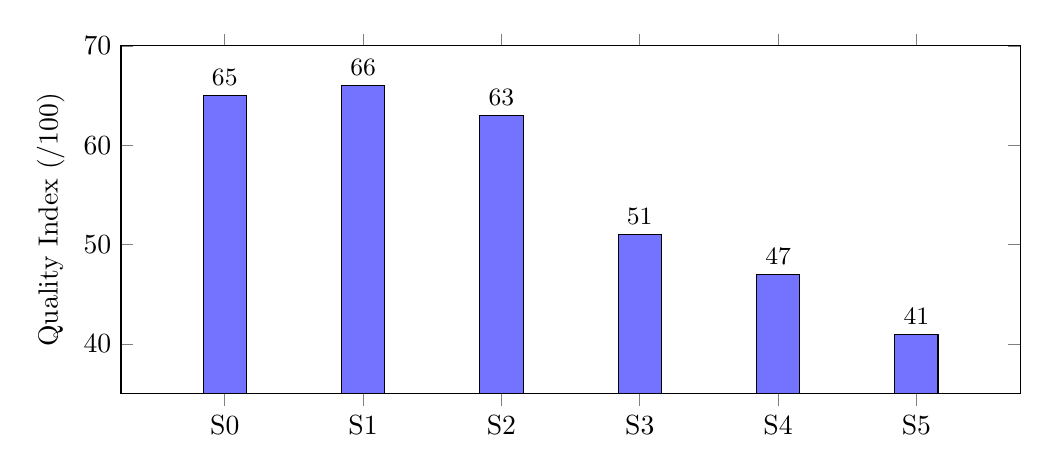
\begin{tikzpicture}
\begin{axis}[
  ybar,
  width=13cm, height=6cm,
  bar width=0.55cm,
  ylabel={Quality Index (/100)},
  ymin=35, ymax=70,
  symbolic x coords={S0,S1,S2,S3,S4,S5},
  xtick=data,
  nodes near coords,
  every node near coord/.append style={font=\small\bfseries},
  enlarge x limits=0.15,
]
\addplot[fill=blue!55] coordinates {(S0,65) (S1,66) (S2,63) (S3,51) (S4,47) (S5,41)};
\end{axis}
\end{tikzpicture}
\caption{Quality Index des stratégies Unstructured KB sur 96 questions --- S1 maximise le rappel, S0 reste le point d'équilibre courant}
\label{fig:kb_strategy_qi}
\end{figure}

\subsubsection{Justification : 20 Documents Sémantiques + 12 Full-text}
\label{sec:max_documents}

Le paramètre \textbf{Max Doc Count} limite le nombre de documents retournés par chaque mode de recherche. Ce nombre est injecté dans le contexte du LLM, qui doit ensuite synthétiser une réponse à partir de ces documents. Un nombre trop élevé sature la fenêtre de contexte et ralentit la réponse ; un nombre trop bas risque de manquer le document pertinent.

\begin{itemize}
  \item \textbf{25 documents sémantiques (S0)} : couvre les reformulations et les questions indirectes tout en gardant le contexte compact. C'est le réglage courant stable.
  \item \textbf{35 documents sémantiques (S1)} : augmente le rappel pour les questions implicites ou mal formulées. Le gain observé est réel mais limité (+1 point), ce qui montre que le rappel supplémentaire apporte aussi du bruit.
  \item \textbf{12 à 15 documents full-text} : assure que les correspondances exactes d'API et de noms de fichiers sont toujours retrouvées. Ce canal est indispensable : le score S5 semantic-only chute à 41/100, preuve que la branche full-text porte une partie majeure de la valeur dans le support STM32.
\end{itemize}

\textbf{Total de documents par requête} : S0 retourne jusqu'à $25 + 12 = 37$ documents, et S1 jusqu'à $35 + 15 = 50$ documents. S1 améliore le rappel mais consomme plus de contexte ; il doit donc être accompagné d'un prompt de synthèse strict pour éviter que le LLM ne mélange plusieurs séries ou périphériques.

\subsubsection{Définition : Search Type (Hybrid)}
\label{sec:search_type}

Le \textbf{Search Type} détermine l'algorithme de recherche utilisé pour interroger la Knowledge Base. La plateforme ST ChatGPT supporte trois modes :

\begin{enumerate}
  \item \textbf{Semantic} : transforme la requête en vecteur (embedding) et recherche les documents les plus proches dans l'espace vectoriel. Comprend le \textit{sens} de la question mais peut rater les termes exacts.
  \item \textbf{Full-text} : recherche par correspondance exacte de mots (BM25/TF-IDF). Trouve les identifiants exacts (\texttt{HAL\_SPI\_TransmitReceive\_DMA}) mais ne comprend pas les reformulations.
  \item \textbf{Hybrid} : exécute les deux recherches en parallèle et fusionne les résultats (union avec déduplication). Combine la compréhension sémantique et la précision lexicale.
\end{enumerate}

Le mode \textbf{Hybrid} a été retenu car les questions des ingénieurs STM32 mélangent systématiquement du langage naturel (``mon SPI crash au deuxième transfert'') et des identifiants techniques exacts (\texttt{HAL\_SPI\_Transmit\_DMA}, \texttt{NUCLEO-H743ZI}).

La Figure~\ref{fig:hybrid_search} schématise la fusion~: la requête est traitée en parallèle par la branche sémantique (embedding AdaV2, seuil 0.55) et la branche full-text (correspondance exacte), puis les deux ensembles de documents sont fusionnés et dédupliqués avant d'être injectés dans le contexte de GPT-5.1.

\begin{figure}[H]
\centering
\begin{tikzpicture}[node distance=0.8cm,
  q/.style={rectangle, draw=gray, fill=codebg, text width=2.6cm, minimum height=0.8cm, align=center, font=\scriptsize\bfseries},
  sem/.style={rectangle, draw=stblue, fill=stlightblue!45, text width=3.2cm, minimum height=0.8cm, align=center, font=\scriptsize},
  ft/.style={rectangle, draw=storange, fill=storange!20, text width=3.2cm, minimum height=0.8cm, align=center, font=\scriptsize},
  fus/.style={rectangle, draw=stgreen, fill=stgreen!15, text width=2.8cm, minimum height=0.8cm, align=center, font=\scriptsize\bfseries},
  arr/.style={-{Stealth[length=2.5mm]}, thick}
]
\node[q] (query) {Requête\\ingénieur};
\node[sem, above right=0.5cm and 1.6cm of query] (sem) {Branche sémantique\\\scriptsize embedding, seuil 0.55, 25 docs};
\node[ft, below right=0.5cm and 1.6cm of query] (ft) {Branche full-text\\\scriptsize match exact API, 12 docs};
\node[fus, right=1.6cm of query, xshift=5.2cm] (fus) {Fusion + déduplication};
\node[q, right=1.4cm of fus, draw=stgreen, fill=stgreen!10] (ctx) {Contexte\\GPT-5.1};
\draw[arr] (query) -- (sem);
\draw[arr] (query) -- (ft);
\draw[arr] (sem) -- (fus);
\draw[arr] (ft) -- (fus);
\draw[arr] (fus) -- (ctx);
\end{tikzpicture}
\caption{Recherche hybride : fusion des branches sémantique et full-text avant génération}
\label{fig:hybrid_search}
\end{figure}

\subsubsection{Tool Description}

La description du tool KB est critique car elle guide le LLM dans sa décision d'appeler ou non le tool :

\begin{quote}
\small\texttt{Retrieve technical knowledge about STM32Cube microcontroller firmware from GitHub repositories. Contains: resolved issues with root cause and fix, HAL/BSP source file documentation, resolver cases (step-by-step troubleshooting), and diagnostic cards (structured fault analysis). Covers series: STM32F4, STM32H5, STM32H7, STM32U5, STM32WL and their driver sub-repos (HAL, CMSIS, BSP). Query this tool when the user asks about: peripheral configuration problems, HAL API behavior, known bugs and workarounds, board-specific issues, firmware package contents, low-power modes, communication protocols, DMA/interrupt issues, or build errors. Use specific technical terms in queries: peripheral names (SPI, I2C, UART, FDCAN, OSPI), HAL function names, error descriptions, board references, and STM32 part numbers.}
\end{quote}

\textbf{Points clés de cette description} :
\begin{enumerate}
  \item \textbf{Énumération explicite du contenu} (issues, files, resolver, diagnostic) → le LLM sait quoi chercher
  \item \textbf{Liste des séries couvertes} → évite les appels pour des séries absentes (L4, G4)
  \item \textbf{Instruction de reformulation} (``Use specific technical terms'') → améliore la qualité des queries envoyées à la KB
  \item \textbf{Exemples de cas d'usage} → le LLM sait \textit{quand} appeler le tool vs répondre directement
\end{enumerate}

\subsection{Configuration du Tool NovaX (Fallback)}

\subsubsection{Problème Identifié}

Lors de l'ajout initial d'un fallback généraliste, le Quality Index a chuté lorsque la persona appelait le fallback au lieu de chercher dans la KB. Le problème n'était pas le modèle lui-même, mais le \textbf{routage} : une description trop large encourage le LLM principal à déléguer trop tôt, ce qui remplace des réponses traçables issues de la KB par des réponses générales.

\begin{quote}
\small\texttt{[Description initiale, trop permissive]} ``I can help with STM32 questions. Forward the user's question.''
\end{quote}

\subsubsection{Fix : NovaX comme Fallback Strictement Secondaire}

Le fallback utilisé est désormais \textbf{NovaX}, un agent STM32 basé sur STM32 Bugzilla et STCommunity Knowledge Articles. Sa description force explicitement la priorité de la KB Unstructured :

\begin{quote}
\small I am an STM32 MCUs smart agent based on STM32 Bugzilla \& STCommunity Knowledge Articles: MPU: STM32MP1 \& MP2 series; Wireless: STM32WB, WBA, WL series; Ultra-lowpower: STM32L0, L1, L4, L4+, L5, U0, U5 series; Mainstream: STM32F0, G0, C0, F1, F3, G4 and C5 series; High Performance: STM32F2, F4, H5, F7, H7 and N6 series; Tools: STM32CubeMX, IDE, Programmer; X-Cube: Graphics, MC, Safety, Audio, EdgeAI. I am a fallback assistant for STM32 firmware questions that are NOT covered by the Knowledge Base. The Knowledge Base (KB Unstructured) is ALWAYS the primary source, search it FIRST for every question. Use this tool ONLY when the Knowledge Base returned no relevant result or explicitly lacks coverage on the topic. Forward the user's exact question without modification. Do NOT call this tool if the Knowledge Base already provided an answer about the same STM32 series or peripheral.
\end{quote}

\textbf{Rôle exact de NovaX} : NovaX n'est pas une source primaire pour les issues GitHub STM32Cube. Il sert à couvrir les questions hors périmètre de la KB : explications générales HAL/LL, middleware (FreeRTOS, lwIP, USB, FatFs), raisonnement STM32CubeMX, limitations matérielles, arbitrages de conception embedded, ou séries/périphériques absents de la KB.

\subsubsection{Impact Mesuré}

\begin{longtable}{lcc}
\toprule
\textbf{Configuration} & \textbf{Quality Index} & \textbf{$\Delta$} \\
\midrule
KB seule / routage KB-first & 65 & baseline courant S0 \\
KB S1 Recall+ / routage KB-first & \textbf{66} & +1 \\
Fallback permissif & dégradé & Court-circuite la KB \\
KB + NovaX restrictif & en validation & Test final S1 en cours \\
\bottomrule
\end{longtable}

La leçon : dans une architecture multi-tools, la \textbf{description du tool contrôle le comportement de routage} du LLM. NovaX doit être appelé uniquement après une recherche KB non concluante. Cette contrainte protège la traçabilité : si la KB contient une issue, un fichier, une diagnostic card ou un resolver case pertinent, la réponse doit rester ancrée dans ces documents.

\subsection{System Prompt de la Persona}

Le system prompt guide le comportement global de la persona. Les éléments clés :

\begin{enumerate}
  \item \textbf{Identité} : ``You are ST GitHub Analyzer, a technical assistant specialized in STM32Cube MCU firmware.''
  \item \textbf{Priorité KB} : ``ALWAYS search the Knowledge Base FIRST before answering or using any other tool.''
  \item \textbf{Format de réponse} : citations avec liens GitHub, code actionnable, versions spécifiques
  \item \textbf{Stratégie multi-cas} :
  \begin{itemize}
    \item Match direct → citer la source avec URL
    \item Match partiel → diagnostic + workaround candidat
    \item Aucun match → appeler NovaX OU proposer une action concrète
  \end{itemize}
  \item \textbf{Interdiction} : ne jamais dire ``je ne sais pas'' sans avoir cherché dans la KB
\end{enumerate}

\subsection{Évolution Incrémentale du Quality Index}

Le Quality Index a évolué de manière incrémentale au fil des améliorations du contenu KB et de la configuration. Chaque test mesure la qualité des réponses du chatbot sur un jeu de questions techniques.

\subsubsection{Chronologie des Tests}

\begin{longtable}{p{2.4cm}p{5.2cm}ccp{3.2cm}}
\toprule
\textbf{Date} & \textbf{Test} & \textbf{QI} & \textbf{N} & \textbf{Contenu KB} \\
\midrule
20 Avr & H7 Issues seules & 54 & 50 & Issues H7 uniquement \\
20 Avr & H7 Prompt Fix & 57 & 50 & + System prompt optimisé \\
24 Avr & H7 Config Tool Test & 61 & 50 & + Hybrid search calibré \\
28 Avr & H7 + Diagnostic Cards & 94 & 50 & + Resolver Cases + Diag \\
08 Mai & H7 Real Cases ST Community & 88 & 4 & Test sur cas réels forum \\
02 Juin & Test élargi & 83 & 4 & Multi-séries first attempt \\
08 Juin & Multi-séries (H7+F4+H5+U5+WL) & 54 & 52 & 5 séries complètes \\
29 Juin & All series S0 Balanced & 65 & 96 & KB multi-séries, hybrid équilibré \\
30 Juin & All series S1 Recall+ & \textbf{66} & 96 & Seuil 0.45, rappel renforcé \\
30 Juin & All series S2 Precision+ & 63 & 96 & Seuil 0.65, filtrage agressif \\
30 Juin & All series S3 Semantic-heavy & 51 & 96 & Plus de sémantique, moins de full-text \\
01 Juil & All series S4 Fulltext-heavy & 47 & 96 & Plus de full-text, moins de sémantique \\
01 Juil & All series S5 Semantic-only & 41 & 96 & Ablation sans full-text \\
01 Juil & Test final S1 + NovaX & N/A & 96 & En cours au moment de la rédaction \\
\bottomrule
\end{longtable}

La Figure~\ref{fig:qi_config_evolution} visualise l'évolution historique. La Figure~\ref{fig:kb_strategy_qi} isole ensuite l'effet des paramètres Unstructured KB sur le benchmark moderne de 96 questions.

% Graphique QI evolution - exporter depuis draw.io ou Excel
\begin{figure}[H]
\centering
\begin{tikzpicture}
\begin{axis}[
  ybar,
  width=14cm, height=6.5cm,
  bar width=0.5cm,
  ylabel={Quality Index (/100)},
  ymin=0, ymax=100,
  symbolic x coords={Issues 54, Prompt 57, Hybrid 61, DiagCards 94, Real 88, Multi4 83, Multi52 54, S0 65, S1 66},
  xtick=data,
  x tick label style={rotate=30, anchor=east, font=\scriptsize},
  nodes near coords,
  every node near coord/.append style={font=\scriptsize\bfseries},
  enlarge x limits=0.08,
]
\addplot[fill=blue!50] coordinates {(Issues 54,54) (Prompt 57,57) (Hybrid 61,61) (DiagCards 94,94) (Real 88,88) (Multi4 83,83) (Multi52 54,54) (S0 65,65) (S1 66,66)};
\end{axis}
\draw[-{Stealth[length=3mm]}, red, very thick] (5.2,4.8) -- (5.2,5.8) node[above, font=\scriptsize\bfseries, red] {+33 pts};
\end{tikzpicture}
\caption{Évolution du Quality Index au fil des améliorations incrémentales}
\label{fig:qi_config_evolution}
\end{figure}

\textit{Le graphique en barres montre l'évolution : Issues seules (54) $\to$ +Prompt (57) $\to$ +Hybrid (61) $\to$ +Diag Cards (94, $\uparrow$+33) $\to$ Real Cases (88) $\to$ Multi 4Q (83) $\to$ Multi 52Q (54, dilution multi-séries). Le saut majeur de 61 à 94 démontre l'impact des Diagnostic Cards.}

\subsubsection{Analyse de l'Évolution}

\paragraph{Phase 1 : Issues seules (QI = 54)}

Le score initial de 54 avec les issues H7 seules montre que les issues structurées (symptôme, root cause, fix) fournissent déjà une base solide pour le RAG. Les lacunes :
\begin{itemize}
  \item Pas de documentation de fichiers → questions sur les API non couvertes
  \item Pas de chaînes Issue→PR→Commit → pas de traçabilité du fix
  \item Pas de cartes de diagnostic → les problèmes complexes multi-étapes mal couverts
\end{itemize}

\paragraph{Phase 2 : Ajout des Resolver Cases et Diagnostic Cards (QI = 94)}

Le saut de 61 à \textbf{94} est le gain le plus important du projet. Les \textbf{Diagnostic Cards} structurent l'information sous forme :

\begin{quote}
Symptôme → Hypothèses → Validation → Root Cause → Fix → Prévention
\end{quote}

Cette structure correspond exactement à la façon dont un ingénieur raisonne face à un problème embedded. Le retrieval RAG trouve ces cartes car elles contiennent des \textbf{query aliases} (reformulations multiples du problème) et des \textbf{keywords techniques} (noms d'API, registres, erreurs).

Les \textbf{Resolver Cases} ajoutent la dimension de traçabilité :
\begin{quote}
Issue \#42 → PR \#87 → Commit abc123 → Fichier modifié : \texttt{stm32f4xx\_hal\_spi.c}
\end{quote}

\paragraph{Phase 3 : Passage multi-séries (QI = 54)}

Le score chute à 54 lors de l'ajout de 4 nouvelles séries (F4, H5, U5, WL). Cette chute s'explique par :

\begin{enumerate}
  \item \textbf{Dilution du contexte} : la KB passe de $\sim$2\,000 à $\sim$14\,000 documents. Les queries retournent des documents de séries différentes, diluant la pertinence.
  \item \textbf{Questions nouvelles} : le jeu de test passe de 50 à 52 questions, avec 10 questions sur les nouvelles séries pour lesquelles les Diagnostic Cards ne sont pas encore aussi mûres.
  \item \textbf{Conflit de noms} : des API identiques entre séries (ex: \texttt{HAL\_SPI\_Init} existe dans F4 et H7) créent de l'ambiguïté lors du retrieval.
\end{enumerate}

\textbf{Leçon} : le passage à l'échelle nécessite un \textbf{filtrage par série} plus agressif dans les métadonnées des documents, ou un prompt qui pousse la persona à inclure le nom de la série dans ses queries KB.

\subsubsection{Raisonnement de Chaque Amélioration}

\begin{longtable}{p{4cm}p{5cm}p{4cm}}
\toprule
\textbf{Amélioration} & \textbf{Raisonnement} & \textbf{Impact QI} \\
\midrule
System prompt optimisé & Forcer la recherche KB avant toute réponse & +3 (54→57) \\
Hybrid search & Combiner semantic + full-text pour ne rater ni les reformulations ni les identifiants & +4 (57→61) \\
Diagnostic Cards & Structurer les problèmes complexes en cartes raisonnées & +33 (61→94) \\
Resolver Cases & Ajouter la traçabilité Issue→PR→Fix & Inclus dans +33 \\
NovaX restrictif & Empêcher le court-circuit de la KB & Protège le routage KB-first \\
Files V3 (nettoyage) & Réduire le bruit des CMSIS headers & +3 estimé \\
PDF descriptions & Rendre les figures PDF cherchables & +1 estimé \\
\bottomrule
\end{longtable}

\subsection{Automatisation CI/CD et Opérations}
\label{sec:automation_cicd}

L'objectif de l'automatisation est de garantir une mise à jour \textbf{reproductible}, \textbf{traçable} et \textbf{sûre} de la KB \#793, sans dépendre d'interventions manuelles ad hoc. L'architecture retenue sépare l'orchestration cloud (GitHub Actions) et l'exécution réseau ST (runner self-hosted), indispensable pour atteindre l'API interne ST AI Bridge.

\begin{figure}[H]
\centering
\includegraphics[width=0.95\textwidth]{06_cicd_automation.png}
\caption{Automatisation CI/CD : orchestration GitHub Actions et upload KB via runner self-hosted}
\label{fig:cicd_automation}
\end{figure}

\subsubsection{Principe d'Architecture}

Le flux d'exécution suit trois phases :
\begin{enumerate}
  \item \textbf{Prepare} : synchronisation des repos, exécution du pipeline, enrichissements Alfred, génération des exports ST-ready.
  \item \textbf{Validate} : validation des schémas et contrôle des placeholders pour bloquer les livrables incomplets.
  \item \textbf{Upload} : création/alimentation des datasources et publication des artefacts parent + drivers dans la KB.
\end{enumerate}

Cette structuration explicite réduit le risque opérationnel : une erreur de qualité en phase \textit{Validate} arrête la publication avant impact utilisateur.

\subsubsection{Workflow GitHub Actions}

Le workflow principal \texttt{.github/workflows/auto\_update\_kb.yml} implémente :
\begin{itemize}
  \item des déclencheurs \textbf{planifiés} et \textbf{manuels} ;
  \item une préparation des entrées (liste des séries, mode, politiques d'exécution) ;
  \item un \textbf{runner-check} bloquant qui vérifie la disponibilité d'un runner \texttt{self-hosted} ;
  \item une exécution par série avec traçabilité des artefacts ;
  \item un résumé d'exécution en cas de succès ou d'échec.
\end{itemize}

Le contrôle de disponibilité du runner évite les faux positifs : si aucun runner ST n'est disponible, le workflow échoue explicitement avec un message d'exploitation, plutôt que de terminer en vert sans traitement.

\subsubsection{Script Orchestrateur Unifié}

La brique centrale est \texttt{pipeline\_Automation/workflow/Run\_Single\_Series\_Full\_Pipeline\_And\_Upload.ps1}. Elle unifie la chaîne complète pour une série et fournit trois modes d'exploitation :

\begin{longtable}{p{2.8cm}p{9.4cm}}
\toprule
\textbf{Mode} & \textbf{Comportement} \\
\midrule
\texttt{Full} & Exécute \textit{Prepare + Upload} en one-shot (mode standard production). \\
\texttt{Prepare} & Génère et valide les artefacts localement sans publication KB (mode debug et pré-validation). \\
\texttt{Upload} & Publie uniquement des artefacts déjà préparés (mode reprise après incident réseau/API). \\
\bottomrule
\end{longtable}

Commande opérationnelle de référence :
\begin{lstlisting}[language=bash]
.\pipeline_Automation\workflow\Run_Single_Series_Full_Pipeline_And_Upload.ps1 \
  -Series H7 -Mode Full
\end{lstlisting}

\subsubsection{Garde-fous Qualité Avant Publication}

L'automatisation intègre deux verrous critiques :
\begin{enumerate}
  \item \textbf{Validation schéma} : exécution de \texttt{validate\_schemas.py} pour garantir la conformité structurelle des JSON.
  \item \textbf{Placeholder gate} : rejet des livrables contenant encore \texttt{[IMAGE DESCRIPTION UNAVAILABLE]} ou des marqueurs PDF non résolus.
\end{enumerate}

La politique \texttt{PlaceholderPolicy} est paramétrable (\texttt{Fail}, \texttt{Warn}, \texttt{Off}), mais \texttt{Fail} est la valeur recommandée en production pour préserver la qualité perçue des réponses.

\subsubsection{Stratégie d'Upload et Traçabilité}

L'upload vers KB \#793 est réalisé via \texttt{Add\_Data\_Source\_Files.py} selon deux cas :
\begin{itemize}
  \item \textbf{operation new} : création d'une datasource si aucun ID n'est fourni ;
  \item \textbf{operation add} : ajout dans une datasource existante quand l'ID est connu.
\end{itemize}

Le script publie les artefacts du repo parent puis ajoute les sorties \texttt{drivers/*} dans les datasources parentes correspondantes (issues, files, resolver, diagnostic). Cette approche maintient une séparation logique par série tout en conservant une base unifiée côté exploitation.

Les IDs effectifs sont sauvegardés dans :
\begin{lstlisting}[language=bash]
datasets/07_delivery/st_ready/by_series/<serie>/upload_datasource_ids_<serie>.json
\end{lstlisting}

et synchronisés dans \texttt{shared/config/config\_all\_series.json} pour assurer la continuité entre les exécutions.

\subsubsection{Runbook Opérateur (Production)}

Le runbook recommandé est :
\begin{enumerate}
  \item Lancer d'abord \texttt{Prepare} sur la série cible.
  \item Vérifier les \texttt{summary\_*.json}, la validation schéma et l'absence de placeholders.
  \item Lancer \texttt{Full} (ou \texttt{Upload} si les artefacts sont déjà prêts).
  \item Contrôler les IDs sauvegardés et la cohérence des datasources créées/alimentées.
\end{enumerate}

Cette discipline d'exploitation est essentielle pour les soutenances internes : elle permet de démontrer à la fois la robustesse technique et la gouvernance de la chaîne de livraison.

\subsection{Couverture Actuelle et Future}
\label{sec:couverture}

\subsubsection{13 Séries en Production}

Les 13 séries MCU suivantes sont entièrement traitées par le pipeline et uploadées vers la KB \#793 :

\begin{longtable}{lcccccc}
\toprule
\textbf{Série} & \textbf{Repos} & \textbf{Issues} & \textbf{Files} & \textbf{Resolver} & \textbf{Diag.} & \textbf{Alfred} \\
\midrule
STM32CubeC0 & 4 & \checkmark & \checkmark & --- & \checkmark & \checkmark \\
STM32CubeF0 & 5 & \checkmark & \checkmark & --- & \checkmark & \checkmark \\
STM32CubeF1 & 6 & \checkmark & \checkmark & \checkmark & \checkmark & \checkmark \\
STM32CubeF2 & 4 & \checkmark & \checkmark & --- & \checkmark & \checkmark \\
STM32CubeF3 & 5 & \checkmark & \checkmark & --- & \checkmark & \checkmark \\
STM32CubeF4 & 16 & \checkmark & \checkmark & \checkmark & \checkmark & \checkmark \\
STM32CubeF7 & 8 & \checkmark & \checkmark & \checkmark & \checkmark & \checkmark \\
STM32CubeG0 & 5 & \checkmark & \checkmark & --- & \checkmark & \checkmark \\
STM32CubeH5 & 6 & \checkmark & \checkmark & \checkmark & \checkmark & \checkmark \\
STM32CubeH7 & 12 & \checkmark & \checkmark & \checkmark & \checkmark & \checkmark \\
STM32CubeH7RS & 4 & \checkmark & \checkmark & --- & \checkmark & \checkmark \\
STM32CubeU5 & 8 & \checkmark & \checkmark & \checkmark & \checkmark & \checkmark \\
STM32CubeWL & 5 & \checkmark & \checkmark & \checkmark & \checkmark & \checkmark \\
\bottomrule
\end{longtable}

\textit{Note : ``---'' pour Resolver signifie que les issues de cette série n'ont pas de chaînes Issue$\to$PR$\to$Commit complètes, pas que le pipeline ne supporte pas le format.}

\subsubsection{4 Nouvelles Séries Exportées (Pipeline Terminé)}

Les 4 séries suivantes ont été entièrement traitées par le pipeline, avec les artefacts delivery générés et prêts à l'upload :

\begin{longtable}{lccccc}
\toprule
\textbf{Série} & \textbf{Issues} & \textbf{Files} & \textbf{Resolver} & \textbf{Diag. Cards} & \textbf{Statut} \\
\midrule
STM32CubeG4 & 89 & 3\,875 & 0 & 4 & Prêt à uploader \\
STM32CubeL0 & 23 & 2\,614 & 2 & 3 & Prêt à uploader \\
STM32CubeL1 & 11 & 2\,847 & 0 & 3 & Prêt à uploader \\
STM32CubeL4 & 68 & 5\,231 & 1 & 8 & Prêt à uploader \\
\bottomrule
\end{longtable}

\textbf{Observations} :
\begin{itemize}
  \item \textbf{G4 (0 Resolver)} : les 89 issues G4 ont été fermées sans PRs formelles liées. Les corrections ont été intégrées dans des releases globales sans lien explicite issue$\to$PR.
  \item \textbf{L4 (5\,231 files)} : c'est la série avec le plus de fichiers parmi les nouvelles, reflétant un écosystème BSP riche (NUCLEO, Discovery, Eval boards).
  \item \textbf{Alfred Images} : 25 images échouées (API 404 intermittent) sur G4, L0, L4. Corrigible par re-run du script d'enrichissement.
\end{itemize}

\subsubsection{8 Séries Configurées (Prêtes à Lancer)}

Les configurations (fichiers \texttt{config\_*.json}) sont créées pour : L5, N6, U0, U3, WB, WB0, WBA, WL3. Le déploiement nécessite :
\begin{enumerate}
  \item Exécution du pipeline : \texttt{python -m pipeline.run\_full\_workflow --export-st-ready}
  \item Création des datasources sur la KB \#793
  \item Upload via les scripts d'automatisation
\end{enumerate}
